\documentclass[12pt,a4paper]{article}
\usepackage{amsmath,amscd,amsbsy,amssymb,latexsym,url,bm,amsthm}
\usepackage{epsfig,graphicx,subfigure}
\usepackage{enumitem,balance}
\usepackage{wrapfig}
\usepackage{mathrsfs,euscript}
\usepackage[usenames]{xcolor}
\usepackage{hyperref}
\usepackage[vlined,ruled,linesnumbered]{algorithm2e}
\hypersetup{colorlinks=true,linkcolor=black}

\newtheorem{theorem}{Theorem}
\newtheorem{lemma}[theorem]{Lemma}
\newtheorem{proposition}[theorem]{Proposition}
\newtheorem{corollary}[theorem]{Corollary}
\newtheorem{exercise}{Exercise}
\newtheorem*{solution}{Solution}
\newtheorem{definition}{Definition}
\theoremstyle{definition}

\renewcommand{\thefootnote}{\fnsymbol{footnote}}

\newcommand{\postscript}[2]
 {\setlength{\epsfxsize}{#2\hsize}
  \centerline{\epsfbox{#1}}}

\renewcommand{\baselinestretch}{1.0}

\setlength{\oddsidemargin}{-0.365in}
\setlength{\evensidemargin}{-0.365in}
\setlength{\topmargin}{-0.3in}
\setlength{\headheight}{0in}
\setlength{\headsep}{0in}
\setlength{\textheight}{10.1in}
\setlength{\textwidth}{7in}
\makeatletter \renewenvironment{proof}[1][Proof] {\par\pushQED{\qed}\normalfont\topsep6\p@\@plus6\p@\relax\trivlist\item[\hskip\labelsep\bfseries#1\@addpunct{.}]\ignorespaces}{\popQED\endtrivlist\@endpefalse} \makeatother
\makeatletter
\renewenvironment{solution}[1][Solution] {\par\pushQED{\qed}\normalfont\topsep6\p@\@plus6\p@\relax\trivlist\item[\hskip\labelsep\bfseries#1\@addpunct{.}]\ignorespaces}{\popQED\endtrivlist\@endpefalse} \makeatother

\begin{document}
\noindent

%========================================================================
\noindent\framebox[\linewidth]{\shortstack[c]{
\Large{\textbf{Lab02-Divide and Conquer}}\vspace{1mm}\\
CS214-Algorithm and Complexity, Xiaofeng Gao, Spring 2021.}}
\begin{center}
\footnotesize{\color{red}$*$ If there is any problem, please contact TA Haolin Zhou. }

\footnotesize{\color{blue}$*$ Name:\underline{Xin Xu}  \quad Student ID:\underline{519021910726} \quad Email: \underline{xuxin20010203@sjtu.edu.cn}}
\end{center}

\begin{enumerate}
\item
    \textit{Recurrence examples.} Give asymptotic upper and lower bounds for $T(n)$ in each of the following recurrences. Assume that $T(n)$ is constant for sufficiently small $n$. Make your bounds as tight as possible.
\begin{enumerate}
	\item $T(n)=4 T(n / 3)+n \log n$
	\item $T(n)=4 T(n / 2)+n^{2} \sqrt{n}$
	\item $T(n)=T(n-1)+n$	
	\item $T(n)=2T(\lfloor \sqrt n\rfloor)+\log n$
\end{enumerate}
\begin{solution}
    We can figure out the time complexity bu the tool of Master Theorem.
	\begin{enumerate}
        \item Since $\log n < n^a$ for any real number $a>0$, by the Master Theorem, $a=4,b=3,d is a little greater than 1$. So, $d< \log_3 4$, and $T(n)=O (n^{\log_3 4})$.
        \item By the Master Theorem, $a=4, b=2, d=5/2$. So, $d>\log_b a=2$. Thus, $T(n)=O (n^{\frac{5}{2}} )$.
        \item Because of recurrence, $T(n)=T(n-1)+n=T(n-2)+(n-1)+n=T(n-3)+(n-2)+(n-1)+n......=T(1)+2+3+...+(n-2)+(n-1)+n=O(n^2)$.
        \item Without generity, we assume that $n=2^{2^k}$. So, $\log_2 n=2^k,k=\log_2 (\log_2 n)$.
              \\Because of recurrence, $T(n)=2T(n^\frac{1}{2})+\log n=2(2T(n^{\frac{1}{2^2}})+\log \frac{1}{2})+\log n=2^2T(n^\frac{1}{2^2})+2\log n=......=2^kT(2)+k\log n=A\log n+B \log n*\log (\log n)=O(\log n\log (\log n))$.
    \end{enumerate}
\end{solution}
\item
\textit{Divide-and-conquer.} Given an integer array $A[1..n]$ and two integers $lower \le upper$, design an algorithm using \textbf{divide-and-conquer} method to count the number of ranges $(i,j)$ ($1 \leq i \leq j \leq n$) satisfying
$$
    lower \leq \sum_{k=i}^{j}{A[k]} \leq upper.
$$
\textbf{Example:}

Given $A = [1,-1,2]$, $lower = 1$, $upper = 2$, return 4.

The resulting four ranges are $(1,1)$, $(3,3)$, $(2,3)$ and $(1,3)$.

\begin{enumerate}
\item
Complete the implementation in the provided C/C++ source code {\color{blue}(The source code \emph{Code-Range.cpp} is attached on the course webpage)}.
\item
Write a recurrence for the running time of the algorithm and solve it by recurrence tree {\color{blue}(You can modify the figure sources \emph{Fig-RecurrenceTree.vsdx} or \emph{Fig-RecurrenceTree.pptx} to illustrate your derivation)}.
\item
Can we use the Master Theorem to solve the recurrence above? Please explain your answer.
\end{enumerate}
\begin{solution}
    \begin{enumerate}
        \item The .cpp file is in the homework folder.
        \item We assume that the input is $O (n)$ for there are $n$ integers in the array to operate the entry.
              \\Additionally, the time complexity of merge\_count is $T(n)$, which satisfies $T(n)=2T(n/2)+O(n\log n)$.
              \begin{figure}[htbp]
                \centering
                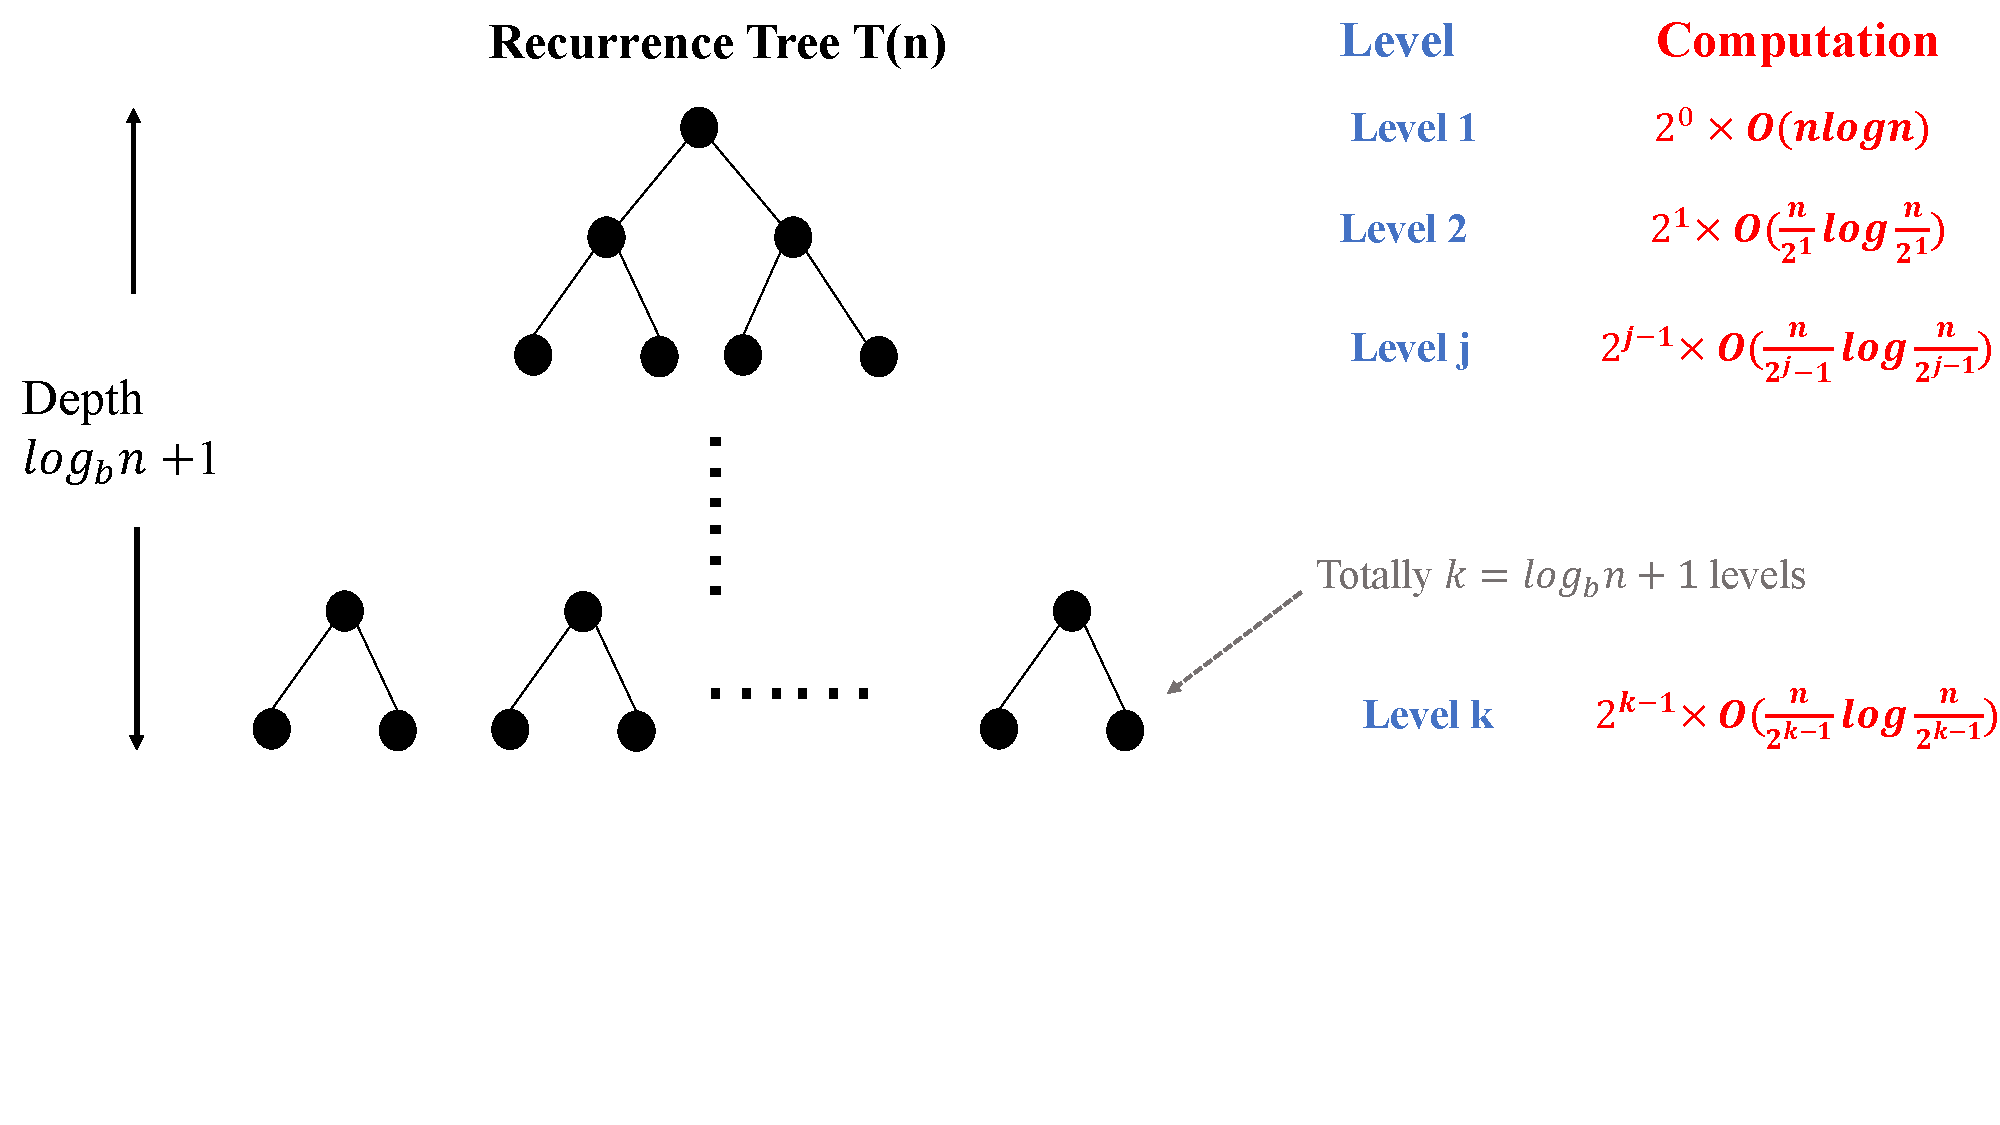
\includegraphics[width=0.4\textwidth]{Fig-RecurrenceTree.pdf}
                \caption{The Recurrence Tree}\label{Fig-RecurrenceTree}
              \end{figure}
              \\Considering that $n=2^k$. With the help of the recurrence Tree, we can figure out that $T(n)=\sum_{i = 0}^{k-1} 2^i \times O (\frac{n}{2^i}\log \frac{n}{2^i} )= \sum_{i = 0}^{k-1} O (2^i \times \frac{n}{2^i}\log \frac{n}{2^i} )= O (n)\sum_{i = 0}^{k-1} \log \frac{n}{2^i} = O(n)\sum_{i=0}^{k-1}(\log n - i\log 2) = O(n\times (\log n)^2) $.
        \item No. If we use the Master Theorem to solve the recurrence above, the output is that $a=2,b=2$, and $\log n$ is smaller than $n^k$ , for any $k >0$, but is greater than $1$. Since we know $O(n)<O(n\log n)$, so we can conclude that $n\log n=n^d, d>1$. And the time complexity $T(n)=O(n\log n)$. This conclusion is contrast from the answer we get above.
              \\ In fact, we just konw $n\log n$ is just a little greater than $n$, and we don't know the exact amount it is.In other words, it's like a boundary. And at this special point, we can't figure out the size between $log_b a$ and $d$. So, we can't use the Master Theorem.
    \end{enumerate}
\end{solution}
\item
\textit{Transposition Sorting Network.} A comparison network is a \textbf{transposition network}  if each comparator connects adjacent lines, as in the network in Fig.~\ref{Fig-Transposition}.

\begin{figure}[htbp]
    \centering
    \includegraphics[width=0.4\textwidth]{Fig-Transposition.pdf}
    \caption{A Transposition Network Example}\label{Fig-Transposition}
\end{figure}

\begin{enumerate}
\item Prove that a transposition network with $n$ inputs is a sorting network if and only if it sorts the sequence $\langle n, n-1, \cdots, 1 \rangle$. {\color{blue}(Hint: Use an induction argument analogous to the \emph{Domain Conversion Lemma}.)}
\item {\color{red}{(Optional Sub-question with Bonus)}} Given any $n \in \mathbb{N}$, write a program using Tkinter in Python to draw a figure similar to Fig.~\ref{Fig-Transposition} with $n$ input wires.
\end{enumerate}
\end{enumerate}
\begin{solution}
    I just finish the first question.
    \begin{enumerate}[label=(\alph*)]
        \item  
              \begin{proof}
                $\Rightarrow$: If a transposition network with $n$ puts is a sorting network, it's obvious that it can sort the sequence <$n, n-1,...,1$> because of the definition of sorting network.
                \\$\Leftarrow$: To improve it, we could use the method of induction.
                \\\textbf{basic step.} For any inputs <$a_1,a_2$> to a comparator, there is a monotonically increasing function $f$ which maps <$1,2$> to <$a_1,a_2$> : $f(2)$=max($a_1,a_2$), $f(1)$=min($a_1,a_2$). According to Domain Conversion Lemma, since the transposition network can sort <$1,2$>, it can also sort <$a_1,a_2$> just with the replace of elements.
                \\\textbf{hypothesis.} For any depth $d< k, k\geqslant 1$, the network can sort sequence <$a_n,a_{n-1},...,a_1$>.
                \\\textbf{induction.} For a comparator with the depth $d=k$ and inputs of <$a_i,a_j$>, it's also true because of our \textbf{basic step.} So, we can claim the statement: if a transposition network can sort the sequence <$n,n-1,...,1$>, it's a sorting network.
              \end{proof}
        \item I'm sorry I can't finish it on time.
    \end{enumerate}
\end{solution}
%========================================================================
\end{document}
